\documentclass[12pt]{article}
%Had an issue with too many packages so needed to put this in to work around it.
\usepackage{etex}

\usepackage{amssymb,amsmath,amsthm,mathtools}
\usepackage{hyperref,cleveref}
\usepackage[margin=1.25in]{geometry}
\usepackage{graphicx,ctable,booktabs} 
\usepackage[parfill]{parskip} % begin paragraphs on empty line rather than indent
\usepackage{fancybox}
\usepackage{tipa} % for \textpipe
\usepackage{caption}
\usepackage{subcaption}
\usepackage{bbm}


\usepackage{tikz}
\usetikzlibrary{shapes,arrows,positioning}

\usepackage{epstopdf} % eps to pdf, declare graphics
\usepackage{soul} % enable highlighting text: use \hl{your text here}
\DeclareGraphicsRule{.tif}{png}{.png}{`convert #1 `dirname #1`/`basename #1 .tif`.png}
\def\thesection{\arabic{section}} % adjust section and subsection labelling 
\def\thesubsection{\arabic{section}(\alph{subsection})}
\makeatletter
\newenvironment{pr}{\@startsection % section as pr
       {section}{1}
       {0.4em}{-.5ex plus -1ex minus -.2ex}{.5ex plus .2ex}
       {\pagebreak[3]\large\bf\noindent{Problem}}}
       {\nopagebreak[3]\vspace{3ex}}
\newenvironment{pa}{\@startsection % subsection as pa
       {subsection}{2}
       {0.3em}{0ex plus -1ex minus -.2ex}{.5ex plus .2ex}
       {\pagebreak[3]\large\noindent{}}}
       {\nopagebreak[3]\vspace{3ex}}
\makeatother
\usepackage{fancyhdr}
\pagestyle{fancy}
\lhead{\footnotesize Adrien Fallou} % header left
\chead{\footnotesize} % header center
\rhead{\thepage} % header right
\lfoot{} 
\cfoot{} 
\rfoot{} 
\renewcommand{\headrulewidth}{.3pt} 
\renewcommand{\footrulewidth}{.3pt}
\setlength\voffset{-0.25in}
\setlength\textheight{648pt}

\setlength{\tabcolsep}{8pt}

\setlength{\parindent}{1cm}
\renewcommand{\arraystretch}{1.2}
% big-O notation
\newcommand{\bigO}[1]{\ensuremath{\mathop{}\mathopen{}\mathcal{O}\mathopen{}\left(#1\right)}}
%%%%%%%%%%%%%%%%%%%%%%%%%%%%%%%

%%%%%%%%%%%%%%%%%%%%%%%%%%%%%%
% Code blocks formatting
\usepackage{listings}
\usepackage{color}

\definecolor{dkgreen}{rgb}{0,0.6,0}
\definecolor{gray}{rgb}{0.5,0.5,0.5}
\definecolor{mauve}{rgb}{0.58,0,0.82}

\lstset{frame=tb,
  language=matlab,
  aboveskip=3mm,
  belowskip=3mm,
  showstringspaces=false,
  columns=flexible,
  basicstyle={\scriptsize\ttfamily},
  numbers=none,
  numberstyle=\tiny\color{gray},
  keywordstyle=\color{blue},
  commentstyle=\color{dkgreen},
  stringstyle=\color{mauve},
  breaklines=true,
  breakatwhitespace=true,
  tabsize=3
}

\makeatletter
\newenvironment{CenteredBox}{% 
\begin{Sbox}}{% Save the content in a box
\end{Sbox}\centerline{\parbox{\wd\@Sbox}{\TheSbox}}}% And output it centered
\makeatother

%%%%%%%%%%%%%%%%%%%%%%%%%%%%%%
\begin{document}

  \title{CS 229 : Project progress report}
  \author{D.Deriso, N. Banerjee, A. Fallou}
  \date{\today}
  \maketitle
  \thispagestyle{empty}
  %%%%%%%%%%%%%%%%%%%%%%%%%%%%%%%

\section*{Introduction}
%
\small  
Our aim is to predict the pulse oximeter waveform of a person purely from a video of them. 
This would give us both the heart rate and the $O_2$ saturation of the blood without the need for medical equipment.

Why we think this can work will be justified briefly in two steps. 
The first comes from a paper released in 2011 from the MIT Computer Science and Artifical Intelligence Lab. 
They use a procedure called Eulerian Video Magnification \footnote{http://people.csail.mit.edu/mrub/vidmag/},
demonstrating that a person's rate can be extracted from a video by correctly amplifying colors.

The second part of the justification is that pulse oximetry as a technique relies on the change in colour of skin. 
Oxygenated and de-oxygenated blood have slightly different hues of red.
This is caused by the difference in hemoglobin levels and this color difference is what the pulse oximeter looks for. 
We intend to look for this change too.

We believe these two ideas imply that there is information present in the video to reconstruct the pulse oximeter waveform.\\
\\
\\
\section{Getting started}

  We first set out to understand the details of the Eulerian Video Magnification (EVM) process. The video can undergo different treatments depending on the goal, but the process to amplify changes 
  can be summarized as:

  \begin{itemize}
    \item Separate the video into several spatial frequency bands.
    \item In each spatial frequency band, blur and downsample several times. The goal of the first step was to retain important spatial features when going through this second step (e.g. high frequencies such as edges).
    \item Amplify selected temporal frequency band.
    \item Recombine spatial frequencies, and add the result to the original video.
  \end{itemize}
  Figure 1 presents an example for the output of the next-to-last-step. 

  \begin{figure}
    \begin{subfigure}{.5\textwidth}
      \captionsetup{justification=centering}
      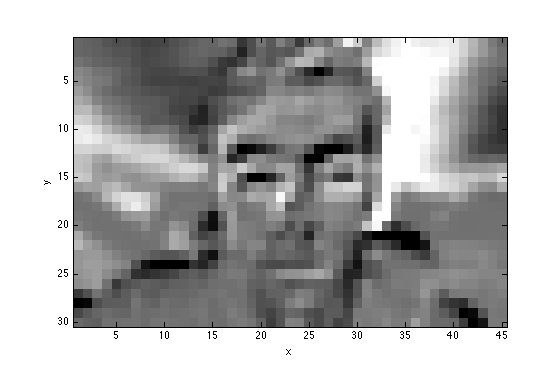
\includegraphics[width=\textwidth]{images/red_peak.png}
      \caption{At at a given time}
    \end{subfigure}
    \begin{subfigure}{.5\textwidth}
      \captionsetup{justification=centering}
      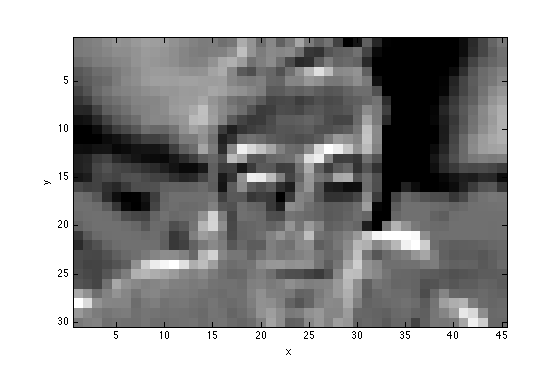
\includegraphics[width=\textwidth]{images/red_trough.png}
      \caption{Half a heartbeat period later}
    \end{subfigure}
    \captionsetup{justification=centering}
    \caption{Red channel of the EVM output, before recombining with the original video.}
  \end{figure}

  Strinkingly, these two frames show that the whole video presents a  periodic color with a frequency 
  that seems equal to the heartbeat. This does not happen with the data provided in the paper, 
  where in a similar video only the person's face changes color.

  Thus, while the EVM processing shows that it is possible to extract medically relevant data from a simple video, we also realized that processing had too many 
  unknown effects for us to get started by directly adding new layers on top of it. Thus we decided to start building from the ground up.

  \section{Understanding our problem}

  What we are essentially trying to do is to get the same reading a pulse oximeter, but with a camera.
  An transmittance pulse oximeter measures the absorption of light by a thin layer of 
  tissue through time. Because oxygenated and de-oxygenated hemoglobin do not absorb light 
  at the same wavelength, this measure yields the blood's oxygen saturation, And by measuring the 
  periodic change of absorbance caused by the pulse, the same measure also yields a heartbeat reading.

  Thus, we could see our experiment as one big pulse oximeter. The room is our light source, 
  the camera our sensor. It happens that we have a video of a whole face, instead we could 
  have only one pixel of the whole video and the concept would still work. 
  The difficulty comes from the fact that, contrary to a an actual pulse oximeter,
  we do not know much about either our light source or our sensors.
  Thus, our problem could be summarized as: matching the red, green and blue channel 
  values of our video to the intensity readings of the pulse oximeter.

\section{Parametrization}
  This new understanding of our problems naturally means that our core set of predictors are the three color channel intensity values through
  time \(I_R(t), I_G(t), I_B(t)\), which are in infinite-dimensional spaces, and we want to do a regression of the reading of our pulse oximeter $Ox(t)$ 
  on these intensity values.
  We then made two additional assumptions that simplify our problem greatly:
  \begin{itemize}
    \item We're only interested in periodic phenomena.
    \item These phenomena have a frequency lying in the 0-5Hz range.
  \end{itemize}

  The first assumption means we can take Fourier series decomposition of our intensity/oximetry values, the second that we can
  limit the decomposition to only a small number $p$ of harmonics. We took 10 as a starting value:
  \[
    I(t)/Ox(t) = \sum_{n=-p}^{p} c_n e^{i \left(\frac{2\pi nt}{T}  + \phi_n \right) }
  \]

  Thus, our training output $y$ is a vector of size $2p$, with the coefficients of the Fourier decomposition.
  Our feature vector contains the $2p$ coefficients of the Fourier decomposition for each of the three color channels.
  Each pixel is considered a different training example, we have $k$ of them for one video (typically \(k=1280\times 720\)).
  Thus our parameters matrix, $\theta \in \mathbb{R}^{(3p) \times k}$


\section{Initial results}
  Our initial computations on the pixel-intensity data revealed, unsuprisingly,
  that pixel intensity variation over time for a reasonably still video was not large.
  Often a single color channel for a pixel would have a range of 3 (when it could vary from 0-255) over the whole video, even if that pixel was contained in the face.
  The DFT of the data would produce large peaks at 0 Hz and would rapidly diminish in magnitude. Because of this, we haven't hade any significant linear regression results.
  A simple solution is to subtract a mean intensity value to our pixel, so as to increase the relative intensity variations.
  Ultimately, we may have to resort to using EVM-enhanced videos if our training data has signals that are too weak to pick up.


  %%%%%%%%%%%%%%%%%%%%%%%%%%%%%%%
\end{document}


